\documentclass[UTF8]{ctexart}
\usepackage{amsmath}
\usepackage{graphicx}
\usepackage{hyperref}
\usepackage{tabularx}
\usepackage{booktabs}
\usepackage{geometry}
\usepackage{array}

\geometry{a4paper, margin=1in}

\title{Modbus RTU Learning based on RS485}
\author{倪煜晖}
\date{\today}

\begin{document}

\maketitle

% 生成目录
\tableofcontents

\section{说明}
记录Modbus RTU通讯协议学习过程,用于实现xArm6机械臂与知行机器人夹爪之间的通信,以备后续查看使用。

\section{Modbus RTU与 RS485初探}

\subsection{简介}
Modbus是一种应用协议,RTU是一种通信模式,而RS485是总线串行标准。前二者工作在应用层与链路层,而RS485工作在物理层。

\subsection{联系与区别}
\begin{itemize}
    \item Modbus RTU:一种主从通信协议。它定义了数据传输的规则,包括数据帧的格式、帧的开始和结束标志、地址域、功能码、数据区和错误检测域等。例如,在一个 Modbus RTU 帧中,地址域用于标识从设备的地址,功能码用于指定主设备希望从设备执行的操作,如读取寄存器、写入寄存器等。
    \item RS485:一种电气接口标准,它规定了数据传输的物理层特性,如信号电平、传输速率、传输距离等。RS - 485 支持多点通信,能够在长距离和高噪声环境下可靠地传输数据。
\end{itemize}

在我们的任务中,RS - 485 提供了硬件层面的通信通道,Modbus RTU 则是在这个通道上运行的协议,规定了数据的传输格式、帧结构等内容,二者相互配合来实现设备之间的通信。

\subsection{重点}
RS485使用差分传输模式,使用双绞线$A,B$之间的电位差来实现通信。它的核心是一个主机与多个从机的通讯。这里需要注意的是,这和$\textbf{I/O}$通信完全没有关系,也就是说,我们$\textbf{I/O}$的五根线大概是没用的。由于RS485协议对电位敏感,建议在之后断开对这五根线的连接,保证接地唯一。后续,还需要考虑使用万用表对串行接口进行检查,确保有电压与信号。


% 插入图片示例
\begin{figure}[htbp]
    \centering
    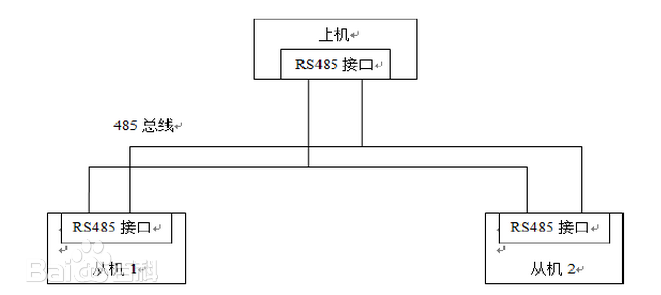
\includegraphics[width=0.8\textwidth]{master_slave.png}
    \caption{一主多从}
    \label{ms}
\end{figure}
确认接线之后,我们把注意力更多放在Modbus RTU上。


\section{使用机器码实现Modbus RTU通信}
\subsection{参数配置}
\subsubsection{夹爪要求}
\begin{itemize}
    \item 波特率: 115200
    \item ID: 默认为1
    \item 数据格式:默认的数据格式为无检验
    \item 校验模式:使用16进制CRC校验码,低字节在前
\end{itemize}

这里highlight校验模式。

使用手册中给出了示例通信码 01 06 01 02 00 64 28 1D。
具体解释会在后面章节注明,也可以直接参照表格\eqref{tab:data_frame}。注意到,这里的最后两位是校验码,由前六位决定。我们遇到的报文无效问题由一部分应该是这个原因。


\begin{table}[htbp]
    \centering
    \caption{数据帧格式说明}
    \label{tab:data_frame}
    \begin{tabularx}{\textwidth}{>{\raggedright\arraybackslash}p{0.15\textwidth} 
                                >{\raggedright\arraybackslash}p{0.1\textwidth} 
                                >{\raggedright\arraybackslash}X 
                                >{\raggedright\arraybackslash}X}
        \toprule
        \textbf{数据} & \textbf{字节} & \textbf{数据说明} & \textbf{备注} \\ 
        \midrule
        01            & 1             & 从机地址           & 0x01 为设备 ID 号,0x00 为广播地址(无回应) \\ 
        \midrule
        06            & 1             & 功能码             & 单个保持寄存器的写入 \\ 
        \midrule
        01 02         & 2             & 数据地址           & 0x0102 为需要执行功能码的数据地址(执行器临时区运动位置) \\ 
        \midrule
        00 64         & 2             & 数据值             & 0x0064 为 16 进制的 100,即将执行器运动位置(临时区)的值设定为 100 \\ 
        \midrule
        28 1D         & 2             & CRC 校验码         & 16 进制 CRC 校验码,低字节在前 \\ 
        \bottomrule
    \end{tabularx}
\end{table}

为了生成正确的校验码,我找到了\href{http://www.ip33.com/crc.html}{生成网站}并且正确生成了校验码。

\begin{figure}[htbp]
    \centering
    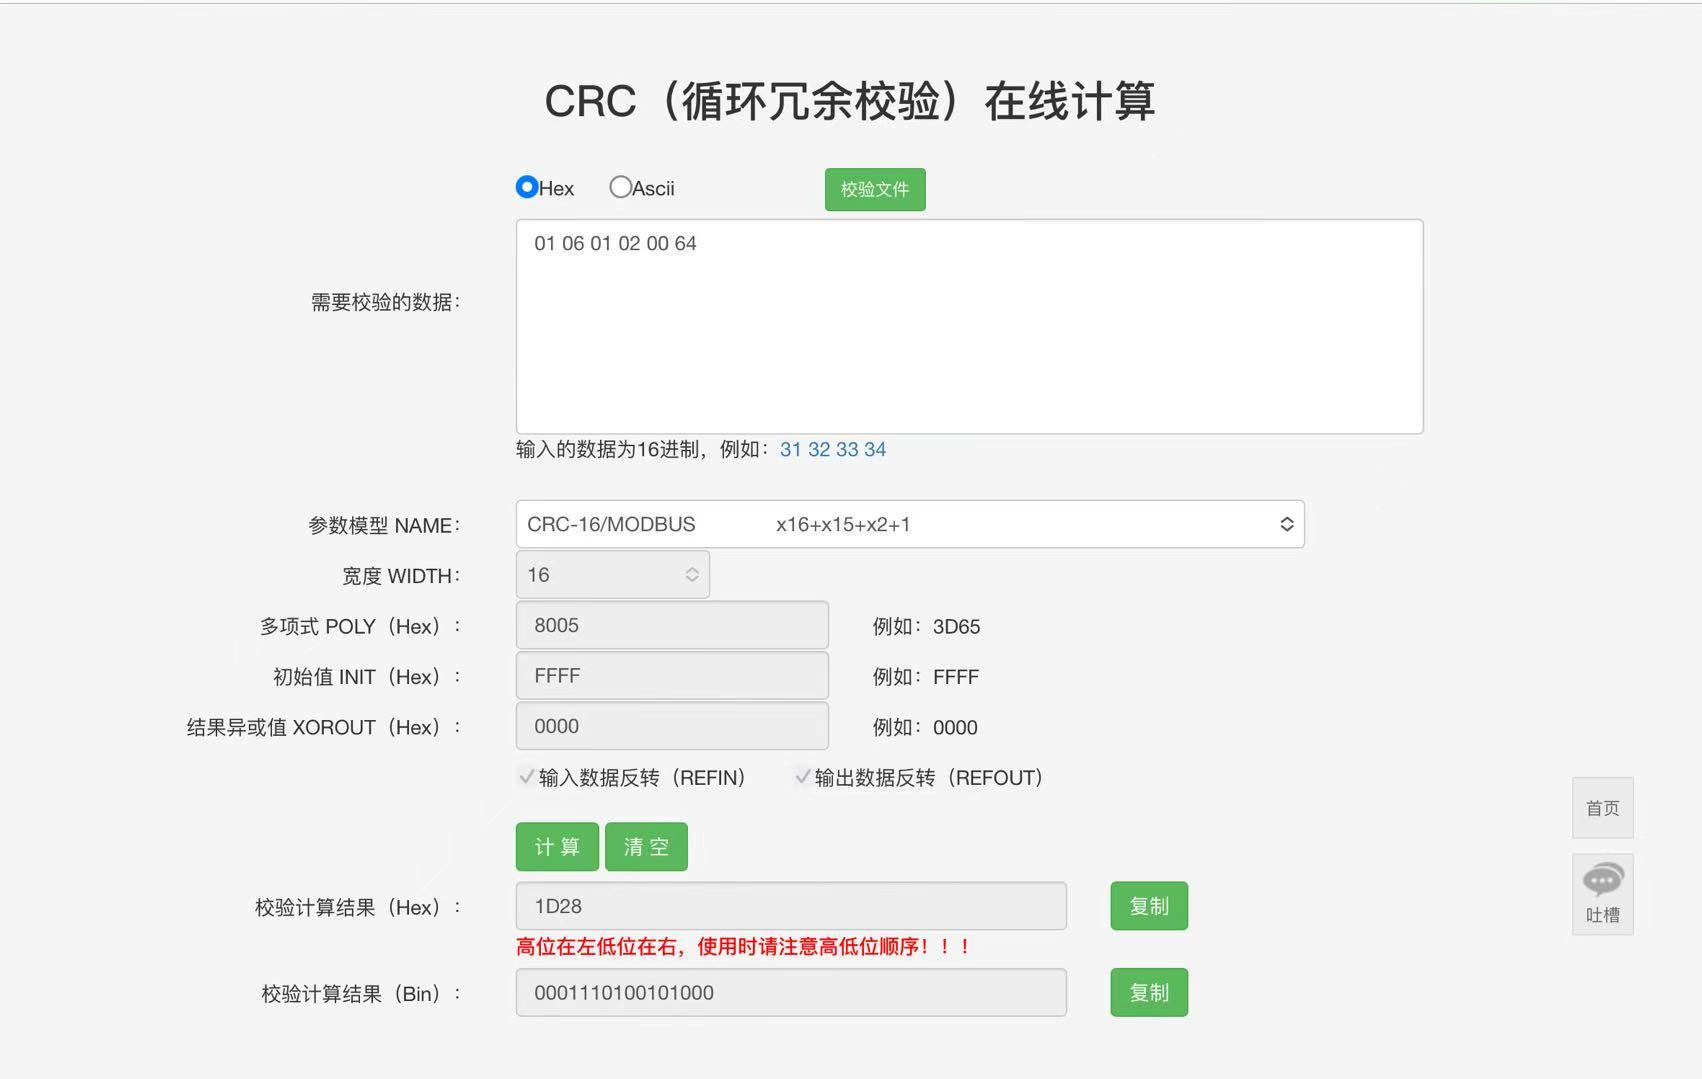
\includegraphics[width=0.8\textwidth]{ip33.jpg}
    \caption{校验码}
    \label{verti}
\end{figure}

值得注意的是,xArm手册中提到自动生成CRC校验码,不知道使用的是否为16位,也不知道采用的是低位在前还是高位在前,可能成为核心问题。

\subsubsection{xArm要求}
\begin{itemize}
    \item 波特率:默认200000
    \item 12位6字节十六进制编码,\bf{自动生成}CRC校验码
\end{itemize}

之前一直无法执行很有可能是位数不对与设备ID不对,应当只输入6字节,选定正确设备ID也就是1,后续尝试。

\subsection{通用Modbus RTU指令}

\begin{table}[h]
    \centering
    \caption{Modbus RTU 数据帧结构}
    \label{tab:modbus_rtu_frame}
    \begin{tabular}{|l|l|l|l|}
    \hline
    \textbf{字段名称} & \textbf{占用字节数} & \textbf{描述} & \textbf{示例} \\ \hline
    从机地址 & 1 & 目标设备的地址,范围为0-255 & 0x01 \\ \hline
    功能码 & 1 & 指示操作类型,例如读取或写入 & 0x03 \\ \hline
    数据区 & 可变 & 根据功能码的不同而变化 & 
    \begin{tabular}{@{}l@{}}
    读保持寄存器时,数据区包含:\\
    起始地址(2字节)和读取数量(2字节)
    \end{tabular} \\ \hline
    校验码 & 2 & CRC校验,用于检测数据传输完整性 & 0x44 0x3C \\ \hline
    \end{tabular}
    \end{table}
    
    \begin{table}[h]
        \centering
        \caption{Modbus RTU 读取类功能码}
        \label{tab:modbus_rtu_read}
        \begin{tabular}{|l|l|l|}
        \hline
        \textbf{功能码} & \textbf{名称} & \textbf{功能描述} \\ \hline
        0x01 & 读线圈寄存器 & 读取一组开关线圈的当前状态(ON/OFF) \\ \hline
        0x02 & 读离散输入寄存器 & 读取一组开关输入的状态(ON/OFF) \\ \hline
        0x03 & 读保持寄存器 & 读取一个或多个保持寄存器的当前值 \\ \hline
        0x04 & 读输入寄存器 & 读取一个或多个输入寄存器的当前值\\ \hline
        0x07 & 读输入状态 & 读取从设备的输入状态 \\ \hline
        0x08 & 读诊断信息 & 读取从设备的诊断信息 \\ \hline
        \end{tabular}
        \end{table}
        
        \begin{table}[h]
        \centering
        \caption{Modbus RTU 写入类功能码}
        \label{tab:modbus_rtu_write}
        \begin{tabular}{|l|l|l|}
        \hline
        \textbf{功能码} & \textbf{名称} & \textbf{功能描述} \\ \hline
        0x05 & 写单个线圈寄存器 & 设置一个单独的线圈状态(ON/OFF) \\ \hline
        0x06 & 写单个保持寄存器 & 写入单个保持寄存器的值\\ \hline
        0x0F & 写多个线圈寄存器 & 批量更新多个线圈的状态 \\ \hline
        0x10 & 写多个保持寄存器 & 写入多个保持寄存器的值 \\ \hline
        0x11 & 写输入寄存器 & 写入单个输入寄存器的值 \\ \hline
        \end{tabular}
        \end{table}
\subsection{夹爪执行器特有参数(TO DO)}
\subsubsection{ 执行器控制指令}
\begin{table}[h]
\centering
\caption{执行器控制指令 (RAM)}
\label{tab:control_instructions_ram}
\begin{tabular}{|l|l|l|l|l|l|}
\hline
\textbf{地址} & \textbf{内容} & \textbf{设定范围} & \textbf{出厂值} & \textbf{生效方式} & \textbf{说明} \\ \hline
0x0100 & 执行器使能 & 0-1 & 1 & 立即生效 & 
\begin{tabular}{@{}l@{}}0:执行器下使能 \\ 1:执行器上使能 \\ 执行器上电默认为使能状态\end{tabular} \\ \hline
0x0102 & 执行器运动位置 high(临时区) & -2147483647 ~ 2147483647 & 0 & 立即生效 & 
\begin{tabular}{@{}l@{}}设置执行器位置,配合(0x0301、0x0302,0x0303、0x0304,0x403,0x0404) \\ 执行器最小位置、执行器最大位置,行程映射最小值,行程映射最大值使用。 \\ 执行器最终位置 = (执行器最大位置-执行器最小位置)/(行程映射最大值-行程映射最小值)*(执行器运动位置 - 行程映射最小值)+ 执行器最小位置\end{tabular} \\ \hline
0x0103 & 执行器运动位置 low(临时区) &  &  &  &  \\ \hline
0x0104 & 执行器运动速度(临时区) & 0-100 & 100 & 立即生效 & 
\begin{tabular}{@{}l@{}}设置执行器运动速度(临时区),配合(0x0305)执行器最大速度使用,对应执行器最大速度百分比。 \\ 执行器运动速度(临时区) =(执行器运动速度(临时区)/100)*执行器最大速度。\end{tabular} \\ \hline
0x0105 & 执行器运动力矩(临时区) & 0-100 & 100 & 立即生效 & 
\begin{tabular}{@{}l@{}}设置执行器运动力矩(临时区),配合(0x0306)执行器最大电流使用,对应执行器最大力矩百分比。 \\ 执行器运动力矩(临时区) =(执行器运动力矩(临时区)/100)*执行器最大力矩。\end{tabular} \\ \hline
0x0106 & 执行器运动加速度(临时区) & 0-100 & 100 & 立即生效 & 
\begin{tabular}{@{}l@{}}设置执行器运动加速度(临时区),配合(0x0307)执行器最大加速度使用,对应执行器最大加速度百分比。 \\ 执行器运动加速度(临时区)=(执行器运动加速度(临时区)/100)*执行器最大加速度。\end{tabular} \\ \hline
0x0107 & 执行器运动减速度(临时区) & 1-100 & 100 & 立即生效 & 
\begin{tabular}{@{}l@{}}设置执行器运动减速度(临时区),配合(0x0308)执行器最大减速度使用,对应执行器最大减速度百分比。 \\ 执行器运动减速度(临时区)=(执行器运动减速度(临时区)/100)*执行器最大减速度。\end{tabular} \\ \hline
0x0108 & 临时区触发 & 0-1 & 0 & 立即生效 & 
\begin{tabular}{@{}l@{}}0:不触发运动 \\ 1:触发运动,以0x0103~0x0106设置的参数运行到0x0102所设置的位置。\end{tabular} \\ \hline
0x010F & 指令更新模式 & 0-1 & 0 & 立即生效 & 
\begin{tabular}{@{}l@{}}0:立即更新数据模式 \\ 1:忽略更新数据模式\end{tabular} \\ \hline
0x0110 & 多段位置运行方式 & 0-2 & 0 & 立即生效 & 
\begin{tabular}{@{}l@{}}0:序列运动(位置指令起始段序号~位置指令终点段序号) \\ 1:循环运动(位置指令起始段序号~位置指令终点段序号) \\ 2:选段运动\end{tabular} \\ \hline
0x0111 & 位置指令起始段序号 & 1-16 & 1 & 立即生效 & 多段位置指令起始段序号 \\ \hline
0x0112 & 位置指令终点段序号 & 1-16 & 0 & 立即生效 & 
\begin{tabular}{@{}l@{}}多段位置终点段序号,与位置指令起始段序号互相制约,需大于等于位置指令起始段序号\end{tabular} \\ \hline
0x0113 & 暂停再启动之后剩余段数处理方式 & 0-1 & 0 & 立即生效 & 
\begin{tabular}{@{}l@{}}0:运行剩余的段 \\ 1:再次从起始段运行\end{tabular} \\ \hline
0x0114 & 多段位置循环次数 & -1-32767 & 0 & 立即生效 & 
\begin{tabular}{@{}l@{}}多段位置循环次数。仅在多段位置运行方式(0x0110)为1时有效。 \\ -1:无限循环\end{tabular} \\ \hline
0x0116 & 多段点位选择 & 1-16 & 1 & 立即生效 & 1-16:选段1-16 \\ \hline
0x0117 & 多段点位触发 & 0-1 & 0 & 立即生效 & 
\begin{tabular}{@{}l@{}}0:无动作 \\ 1:触发多段点位运动\end{tabular} \\ \hline
0x0118 & 多段点位暂停 & 0-1 & 0 & 立即生效 & 
\begin{tabular}{@{}l@{}}0:无动作 \\ 1:暂停多段点位运动\end{tabular} \\ \hline
0x0119 & 执行器运动位置 P1high & -2147483647 ~ 2147483647 & 0 & 立即生效 & 
\begin{tabular}{@{}l@{}}设置执行器多段点位第一段位置,配合(0x0301、0x0302,0x0303、0x0304,0x403,0x0404) \\ 执行器最小位置、执行器最大位置,行程映射最小值,行程映射最大值使用。 \\ 执行器最终位置 = (执行器最大位置-执行器最小位置)/(行程映射最大值-行程映射最小值)*(执行器运动位置 - 行程映射最小值)+ 执行器最小位置\end{tabular} \\ \hline
0x011A & 执行器运动位置 P1low &  &  &  &  \\ \hline
0x011B & 执行器运动速度 P1 & 0-100 & 0 & 立即生效 & 
\begin{tabular}{@{}l@{}}设置执行器多段点位第一段运动速度(临时区),配合(0x0305)执行器最大速度使用,对应执行器最大速度百分比。 \\ 执行器运动速度(临时区) =(执行器运动速度(临时区)/100)*执行器最大速度。\end{tabular} \\ \hline
0x011C & 执行器运动力矩 P1 & 0-100 & 0 & 立即生效 & 
\begin{tabular}{@{}l@{}}设置执行器多段点位第一段运动力矩(临时区),配合(0x0306)执行器最大电流使用,对应执行器最大力矩百分比。 \\ 执行器运动力矩(临时区) =(执行器运动力矩(临时区)/100)*执行器最大力矩。\end{tabular} \\ \hline
0x011D & 执行器运动加速度 P1 & 0-100 & 0 & 立即生效 & 
\begin{tabular}{@{}l@{}}设置执行器多段点位第一段运动加速度(临时区),配合(0x0307)执行器最大加速度使用,对应执行器最大加速度百分比。 \\ 执行器运动加速度(临时区)=(执行器运动加速度(临时区)/100)*执行器最大加速度。\end{tabular} \\ \hline
0x011E & 执行器运动减速度 P1 & 0-100 & 0 & 立即生效 & 
\begin{tabular}{@{}l@{}}设置执行器多段点位第一段运动减速度(临时区),配合(0x0308)执行器最大减速度使用,对应执行器最大减速度百分比。 \\ 执行器运动减速度(临时区)=(执行器运动减速度(临时区)/100)*执行器最大减速度。\end{tabular} \\ \hline
0x011F & 当前段等待时间 P1 & 0-65535 & 0 & 立即生效 & 设置多段点位第一段运行过后的等待时间 \\ \hline
\end{tabular}
\end{table}

\subsubsection{执行器运动参数}
\begin{table}[h]
\centering
\caption{执行器运动参数 (FLASH)}
\label{tab:motion_parameters_flash}
\begin{tabular}{|l|l|l|l|l|l|}
\hline
\textbf{地址} & \textbf{内容} & \textbf{设定范围} & \textbf{出厂值} & \textbf{生效方式} & \textbf{说明} \\ \hline
0x0301 & 执行器最小位置 high & -2147483647 ~ 2147483647 & 0 & 立即生效 & 设置执行器最小位置 \\ \hline
0x0302 & 执行器最小位置 low &  &  &  &  \\ \hline
0x0303 & 执行器最大位置 high & -2147483647 ~ 2147483647 & 0 & 立即生效 & 设置执行器最大位置 \\ \hline
0x0304 & 执行器最大位置 low &  &  &  &  \\ \hline
0x0305 & 执行器最大速度 & 1-10000 & 2000 & 立即生效 & 设置执行器最大速度 \\ \hline
0x0306 & 执行器最大电流 & 1-2000 & 400 & 立即生效 & 设置执行器最大电流 \\ \hline
0x0307 & 执行器最大加速度 & 1-10000 & 1000 & 立即生效 & 设置闭合最大速度 \\ \hline
0x0308 & 执行器最大减速度 & 1-10000 & 1000 & 立即生效 & 设置闭合最大力矩 \\ \hline
0x0309 & 找零最大路程 high & -2147483647 ~ 2147483647 & 10000 & 立即生效 & 设置找零最大路程 \\ \hline
0x030A & 找零最大路程 low &  &  &  &  \\ \hline
0x030B & 找零最大速度 & 0-10000 & 2000 & 立即生效 & 设置找零最大速度 \\ \hline
0x030C & 找零最大电流 & 0-2000 & 380 & 立即生效 & 设置找零最大电流 \\ \hline
0x030D & 找零加速度 & 1-10000 & 2000 & 立即生效 & 设置找零加速度 \\ \hline
0x030E & 找零减速度 & 0-10000 & 2000 & 立即生效 & 设置找零减速度 \\ \hline
0x0310 & 是否上电回零 & 0-1 & 0 & 立即生效 & 
\begin{tabular}{@{}l@{}}0:上电无动作 \\ 1:上电自动回零\end{tabular} \\ \hline
0x0311 & 执行器执行方向 & 0-1 & 1 & 立即生效 & 
\begin{tabular}{@{}l@{}}0:顺时针回零,逆时针夹紧 \\ 1:逆时针回零,顺时针夹紧\end{tabular} \\ \hline
0x0313 & 运动模式 & 0-1 & 0 & 立即生效 & 
\begin{tabular}{@{}l@{}}0:绝对式 \\ 1:增量式\end{tabular} \\ \hline
0x0314 & 堵转处理模式 & 0-1 & 1 & 立即生效 & 
\begin{tabular}{@{}l@{}}0:LH1,力矩到达后继续运行 \\ 1:LH2,力矩到达后停止 \\ 2:LH3,力矩到达后保持当前位置\end{tabular} \\ \hline
\end{tabular}
\end{table}

\subsubsection{执行器运动状态}
\begin{table}[h]
\centering
\caption{执行器运动状态}
\label{tab:motion_status}
\begin{tabular}{|l|l|l|l|l|l|}
\hline
\textbf{地址} & \textbf{内容} & \textbf{设定范围} & \textbf{出厂值} & \textbf{生效方式} & \textbf{说明} \\ \hline
0x0401 & 保存所有参数 & 0-1 & 0 & 上电有效 & 
\begin{tabular}{@{}l@{}}所有参数在修改后,默认断电不会保存参数。若期望重新上电时保持当前设置的参数,则需手动触发当前寄存器。\end{tabular} \\ \hline
0x0402 & 指令回零 & 0-1 & 0 & 立即生效 & 所有参数恢复出厂设置 \\ \hline
0x0403 & 报警复位 & 0-1 & 0 & 立即生效 & 
\begin{tabular}{@{}l@{}}0:不动作 \\ 1:报警复位\end{tabular} \\ \hline
0x0404 & 行程映射最小值 high & -2147483647 ~ 2147483647 & 0 & 立即生效 & 执行器行程最大值 \\ \hline
0x0405 & 行程映射最小值 low &  &  &  &  \\ \hline
0x0406 & 行程映射最大值 high & -2147483647 ~ 2147483647 & 1000 & 立即生效 & 执行器行程最小值 \\ \hline
0x0407 & 行程映射最大值 low &  &  &  &  \\ \hline
0x0409 & 位置误差最大值 & 0-100 & 10 & 立即生效 & 
\begin{tabular}{@{}l@{}}位置误差判断标准。位置到达 = 丨设定位置-实际位置丨≤(位置误差最大值/10)\end{tabular} \\ \hline
0x040D & 原点偏移 high & -2147483647 ~ 2147483647 & 0 & 立即生效 & 
\begin{tabular}{@{}l@{}}若原点设置过大,需更改行程限制低的偏置值,若大过执行器最大行程会报堵转状态\end{tabular} \\ \hline
0x040E & 原点偏移 low &  &  &  &  \\ \hline
0x040F & 原点偏移时间 & 0-65535 & 0 & 立即生效 & 原点偏移的时间 \\ \hline
\end{tabular}
\end{table}

\subsubsectio*{执行器警报状态}
\begin{table}[h]
\centering
\caption{执行器警报状态}
\label{tab:alarm_status}
\begin{tabular}{|l|l|l|l|l|l|}
\hline
\textbf{地址} & \textbf{内容} & \textbf{设定范围} & \textbf{出厂值} & \textbf{生效方式} & \textbf{说明} \\ \hline
0x0601 & 力矩到达 & 0-1 & 0 & 立即生效 (只读) & 
\begin{tabular}{@{}l@{}}0:力矩未到达 \\ 1:力矩到达(与位置到达互斥)\end{tabular} \\ \hline
0x0602 & 位置到达 & 0-1 & 0 & 立即生效 (只读) & 
\begin{tabular}{@{}l@{}}0:位置未到达 \\ 1:位置到达(与力矩到达互斥)\end{tabular} \\ \hline
0x0603 & 速度到达 & 0-1 & 0 & 立即生效 (只读) & 
\begin{tabular}{@{}l@{}}0:速度未到达最大速度 \\ 1:速度到达最大速度\end{tabular} \\ \hline
0x0604 & 执行器准备完成 & 0-1 & 0 & 立即生效 (只读) & 
\begin{tabular}{@{}l@{}}0:执行器运动准备未完成 \\ 1:执行器运动准备完成(执行器准备完成 = 力矩到达 | 位置到达)\end{tabular} \\ \hline
0x0606 & 当前循环次数 & 0-65535 & 0 & 立即生效 (只读) & 多段运动当前循环次数 \\ \hline
0x0607 & 当前运行段数 & 1-16 & 0 & 立即生效 (只读) & 多段运动当前运行段数 \\ \hline
0x0609 & 实时反馈位置信息 high & -2147483647 ~ 2147483647 & 0 & 立即生效 (只读) & 
\begin{tabular}{@{}l@{}}读取执行器实时位置信息 \\ 执行器位置 = (实时反馈位置信息 high << 16 ) + 实时反馈位置信息 low\end{tabular} \\ \hline
0x060A & 实时反馈位置信息 low &  &  &  &  \\ \hline
0x060B & 实时反馈转速信息 & 0-10000 & 0 & 立即生效 (只读) & 读取执行器实时速度信息 \\ \hline
0x060C & 实时反馈电流信息 & 0-2000 & 0 & 立即生效 (只读) & 读取执行器实时力矩信息 \\ \hline
0x060D & 实时反馈位置比例信息 high & -2147483647 ~ 2147483647 & 0 & 立即生效 (只读) & 
\begin{tabular}{@{}l@{}}读取执行器实时位置信息 \\ 执行器位置 = (实时反馈位置信息 high << 16 ) + 实时反馈位置信息 low\end{tabular} \\ \hline
0x060E & 实时反馈位置比例信息 low &  &  &  &  \\ \hline
0x060F & 实时反馈转速比例信息 & 0-32767 & 0 & 立即生效 (只读) & 读取执行器实时速度信息 \\ \hline
0x0610 & 实时反馈电流比例信息 & 0-32767 & 0 & 立即生效 (只读) & 读取执行器实时力矩信息 \\ \hline
0x0612 & 警报信息 & 0-65535 & 0 & 立即生效 (只读) & 
\begin{tabular}{@{}l@{}}0x01:过温警报 \\ 0x02:堵转警报 \\ 0x04:超速警报 \\ 0x08:初始化故障警报 \\ 0x10:超限检测警报 \\ 0x20:夹取掉落警报\end{tabular} \\ \hline
0x0614 & 参数修改标志 & 0-1 & 0 & 立即生效 (只读) & 
\begin{tabular}{@{}l@{}}0:无相关参数修改 \\ 1:可掉电保存的参数修改后且未保存\end{tabular} \\ \hline
\end{tabular}
\end{table}

\subsubsection{执行器产品信息}
\begin{table}[h]
\centering
\caption{执行器产品信息}
\label{tab:product_information}
\begin{tabular}{|l|l|l|l|l|l|}
\hline
\textbf{地址} & \textbf{内容} & \textbf{设定范围} & \textbf{出厂值} & \textbf{生效方式} & \textbf{说明} \\ \hline
0x0801 & 软件版本 & 厂商设置 ASCII 码 & 3 * 2 个字符 &  &  \\ \hline
0x0802 &  &  &  &  &  \\ \hline
0x0803 &  &  &  &  &  \\ \hline
0x0804 & 产品号 & 厂商设置 ASCII 码 & 10 * 2 个字符 &  &  \\ \hline
0x0805 &  &  &  &  &  \\ \hline
0x0806 &  &  &  &  &  \\ \hline
0x0807 &  &  &  &  &  \\ \hline
0x0808 &  &  &  &  &  \\ \hline
0x0809 &  &  &  &  &  \\ \hline
0x080A &  &  &  &  &  \\ \hline
0x080B &  &  &  &  &  \\ \hline
0x080C &  &  &  &  &  \\ \hline
0x080D &  &  &  &  &  \\ \hline
0x0810 & 产品 ID & 厂商设置 16 进制数字 & 8 * 2 个字符 &  &  \\ \hline
0x0811 &  &  &  &  &  \\ \hline
0x0812 &  &  &  &  &  \\ \hline
0x0813 &  &  &  &  &  \\ \hline
0x0814 &  &  &  &  &  \\ \hline
0x0815 &  &  &  &  &  \\ \hline
0x0816 &  &  &  &  &  \\ \hline
0x0817 &  &  &  &  &  \\ \hline
0x0820 & 硬件版本号 & 厂商设置 16 进制数字 & 5 * 2 个字符 &  &  \\ \hline
0x0821 &  &  &  &  &  \\ \hline
0x0822 &  &  &  &  &  \\ \hline
0x0823 &  &  &  &  &  \\ \hline
0x0824 &  &  &  &  &  \\ \hline
\end{tabular}
\end{table}

\subsubsection{系统管理}
\begin{table}[h]
\centering
\caption{系统管理}
\label{tab:system_management}
\begin{tabular}{|l|l|l|l|l|l|}
\hline
\textbf{地址} & \textbf{内容} & \textbf{设定范围} & \textbf{出厂值} & \textbf{生效方式} & \textbf{说明} \\ \hline
0x2001 & 重启 & 0-1 & 0 & 厂商设置 ASCII 码 3 * 2 个字符 &  \\ \hline
0x2003 & 校准 & 0-1 & 0 & 立即生效 &  \\ \hline
0x2005 & 恢复出厂设置 & 0-1 & 0 & 上电生效 &  \\ \hline
\end{tabular}
\end{table}
\section{使用Python调用Modbus RTU(TO DO)}
TO DO

\section{可能的替代方案——I/O控制(TO DO)}
TO DO



\end{document}